\chapter{Data Insights}
\section{Text Data Analysis}
Text data analysis were performed in the training datasets. Analysis like title length based on character frequency, title length based on word frequency were analysed.

\subsection{Title length based on character frequency}
\begin{figure}[H]
    \centering
    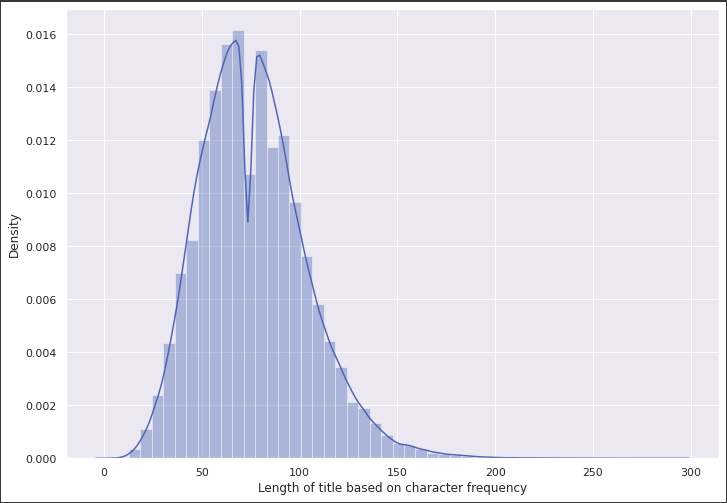
\includegraphics[scale = 0.6]{Basic Analysis/length of title based on character frequency.png}
    \caption{Title length based on number of characters
    (Bi-modal Distribution)}
    \label{fig:Title length based on number of characters}
\end{figure}

From the figure above, it can be deduced that the title length based on number of characters follow bimodal distribution. Its basic statistics value can be observed in following box plot.

\begin{figure}[H]
    \centering
    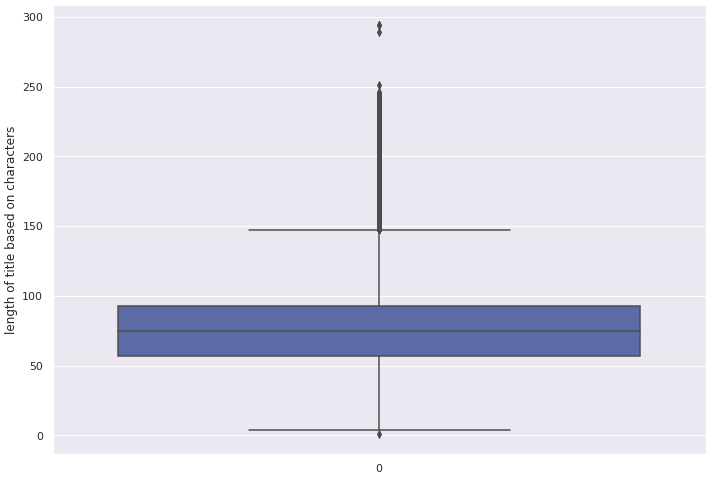
\includegraphics[scale = 0.6]{Basic Analysis/box_plot_length_character.png}
    \caption{Box plot of title length based on character frequency}
    \label{fig:Box plot of title length based on character frequency}
\end{figure}

From the box plot, the average number of characters in a title in the training dataset is found to be 76.3678 $\pm$ 27.2314. The statistics information are shown below.

\begin{table}[H]
    \begin{center}
        \begin{tabular}{ |c|c| }
            \hline
            mean               & 76.3678 \\
            \hline
            standard deviation & 27.2314 \\
            \hline
            minimum            & 1       \\
            \hline
            first quartile     & 57      \\
            \hline
            median             & 75      \\
            \hline
            third quartile     & 93      \\
            \hline
            maximum            & 294     \\
            \hline
        \end{tabular}
    \end{center}
    \caption{Title length statistics based on character frequency}
    \label{table:Title length statistics based on character frequency}
\end{table}

\subsection{Title length based on word frequency}

\begin{figure}[H]
    \centering
    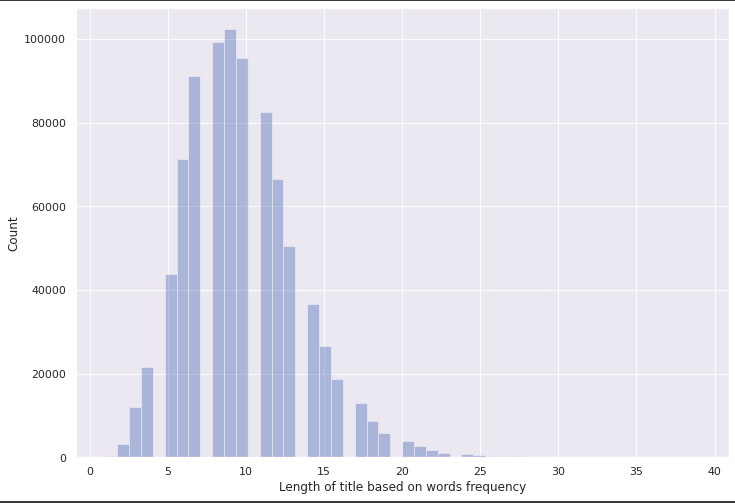
\includegraphics[scale = 0.6]{Basic Analysis/length of title based on word frequency.png}
    \caption{Title length based on word frequency
    (Right Skewed Normal Distribution)}
    \label{fig:Title length based on word frequency}
\end{figure}

From the above distribution plot, it can be deduced that the title length based on word frequency follow right skewed normal distribution.

From the box plot Fig : \ref{fig:Box plot of title length based on word frequency}, the average number of words in a title in the training dataset is found to be 9.7681 $\pm$ 3.6153. The statistics information are shown below.

\begin{table}[H]
    \begin{center}
        \begin{tabular}{ |c|c| }
            \hline
            mean               & 9.7681 \\
            \hline
            standard deviation & 3.6153 \\
            \hline
            minimum            & 1       \\
            \hline
            first quartile     & 7      \\
            \hline
            median             & 9      \\
            \hline
            third quartile     & 12      \\
            \hline
            maximum            & 39     \\
            \hline
        \end{tabular}
    \end{center}
    \caption{Title length statistics based on word frequency}
    \label{table:Title length statistics based on word frequency}
\end{table}

\begin{figure}[H]
    \centering
    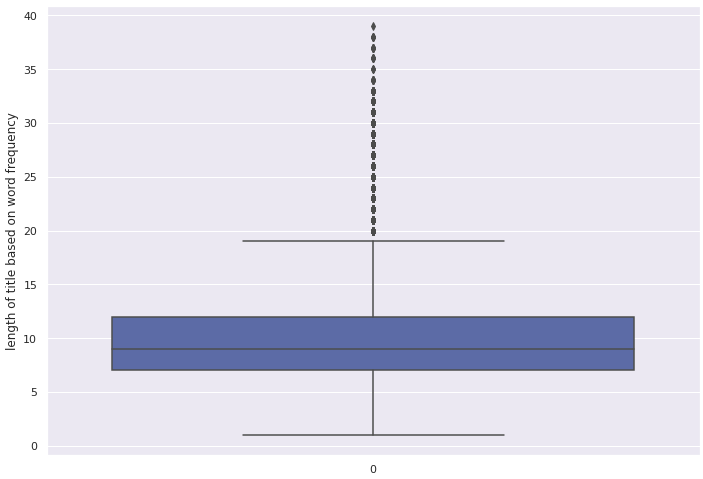
\includegraphics[scale = 0.6]{Basic Analysis/box_plot_length_word.png}
    \caption{Box plot of title length based on word frequency}
    \label{fig:Box plot of title length based on word frequency}
\end{figure}

\section{Word Cloud}
A word cloud (also known as a tag cloud) is a visual representation of words. Cloud creators are used to highlight popular words and phrases based on frequency and relevance. They provide quick and simple visual insights that can lead to more in-depth analyses.

For this report, word cloud is created using the title column of the training data removing all stopwords. From the word cloud Fig \ref{fig:Title Corpus Word Cloud}, we can see the clear dominance of the majority class : cs, math, physics, cond-mat, stat, astro-ph, and quant-ph.

\begin{figure}[H]
    \centering
    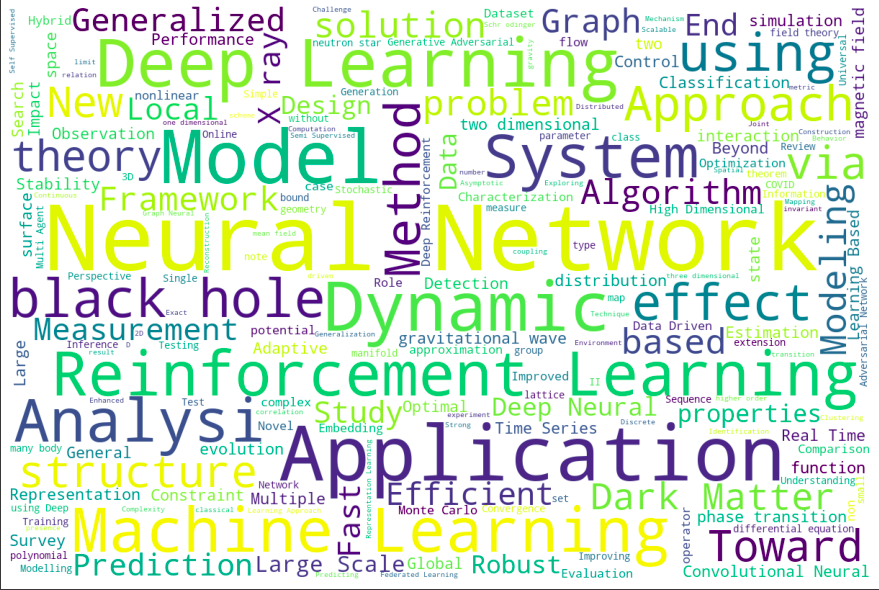
\includegraphics[scale = 0.55]{Word Cloud/300 word cloud.png}
    \caption{Title Word Cloud}
    \label{fig:Title Corpus Word Cloud}
\end{figure}

Let's view the word cloud on specific topics. 

\begin{figure}[H]
    \centering
    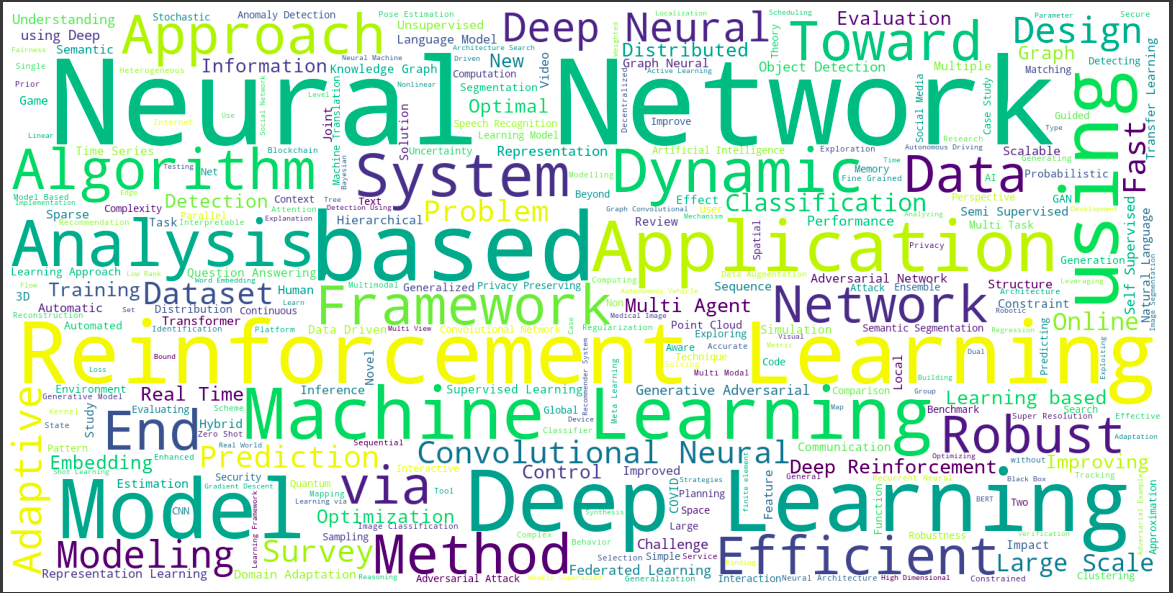
\includegraphics[scale = 0.4]{Word Cloud/cs_word_cloud.png}
    \caption{CS Word Cloud}
    \label{fig:cs Corpus Word Cloud}
\end{figure}

\begin{figure}[H]
    \centering
    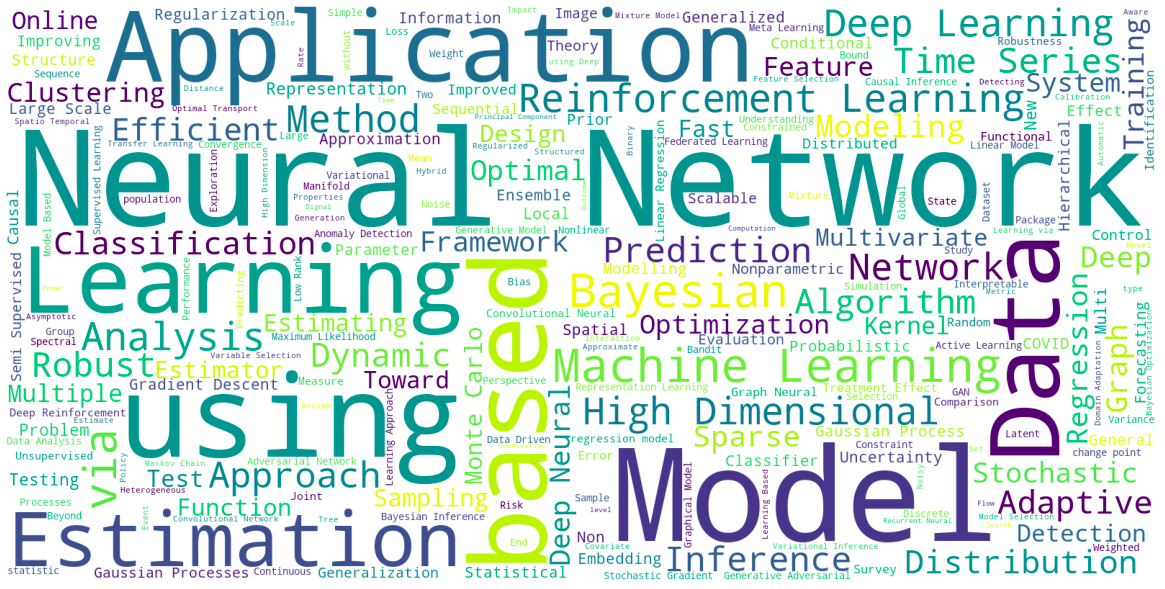
\includegraphics[scale = 0.4]{Word Cloud/stat_word_cloud.png}
    \caption{Stat Word Cloud}
    \label{fig:stat Corpus Word Cloud}
\end{figure}

\begin{figure}[H]
    \centering
    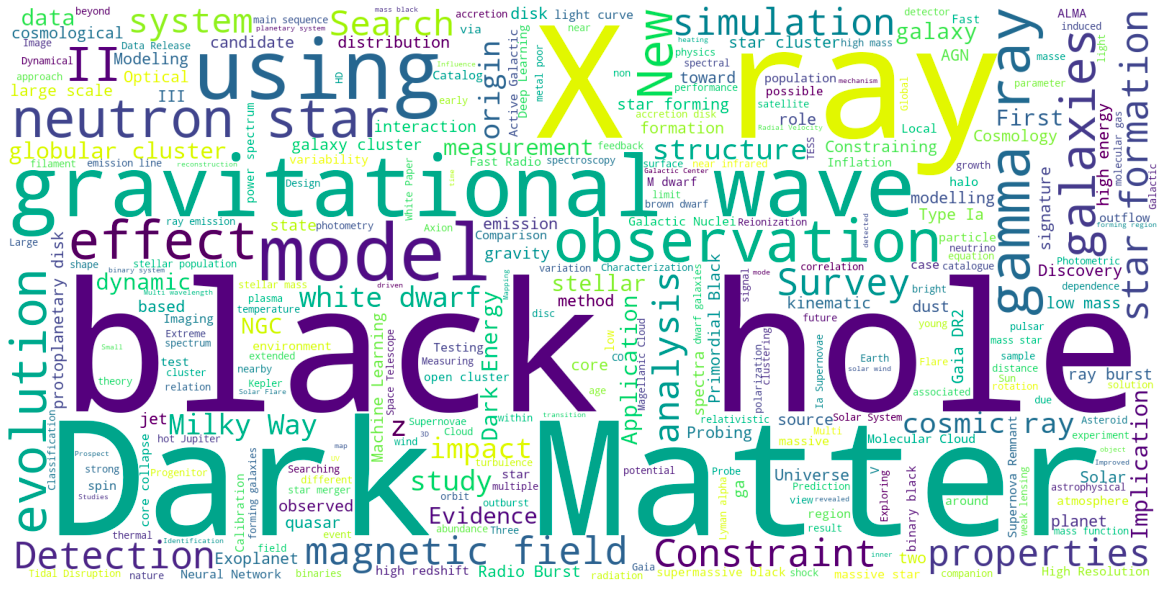
\includegraphics[scale = 0.4]{Word Cloud/astro-ph_word_cloud.png}
    \caption{Astro-ph Word Cloud}
    \label{fig:astro-ph Corpus Word Cloud}
\end{figure}


\begin{figure}[H]
    \centering
    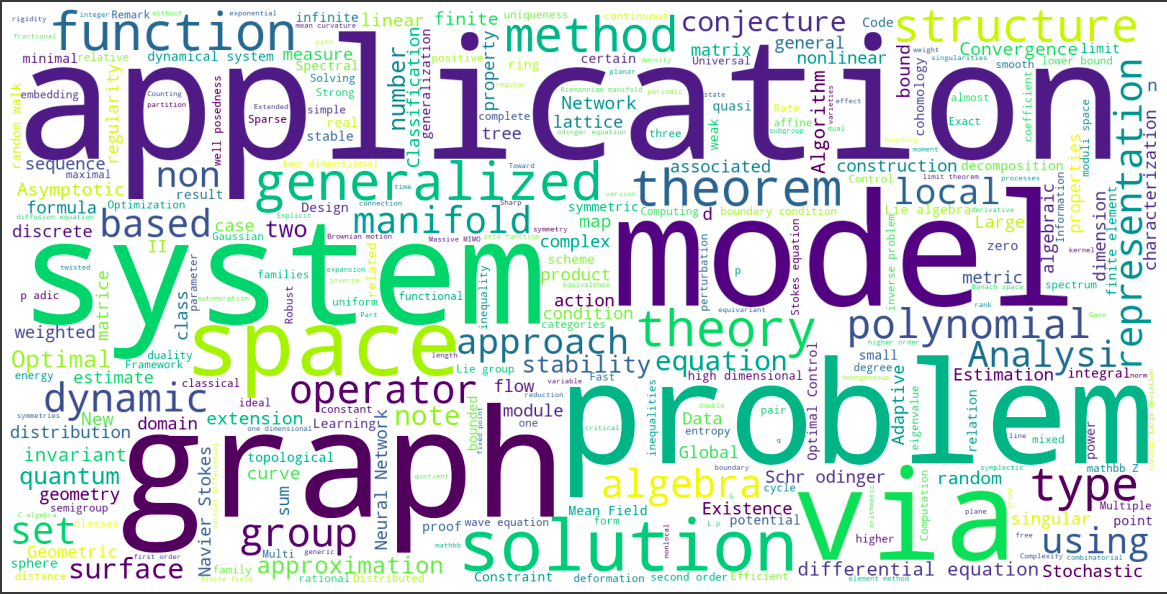
\includegraphics[scale = 0.4]{Word Cloud/math_word_cloud.png}
    \caption{Math Word Cloud}
    \label{fig:math Corpus Word Cloud}
\end{figure}

\begin{figure}[H]
    \centering
    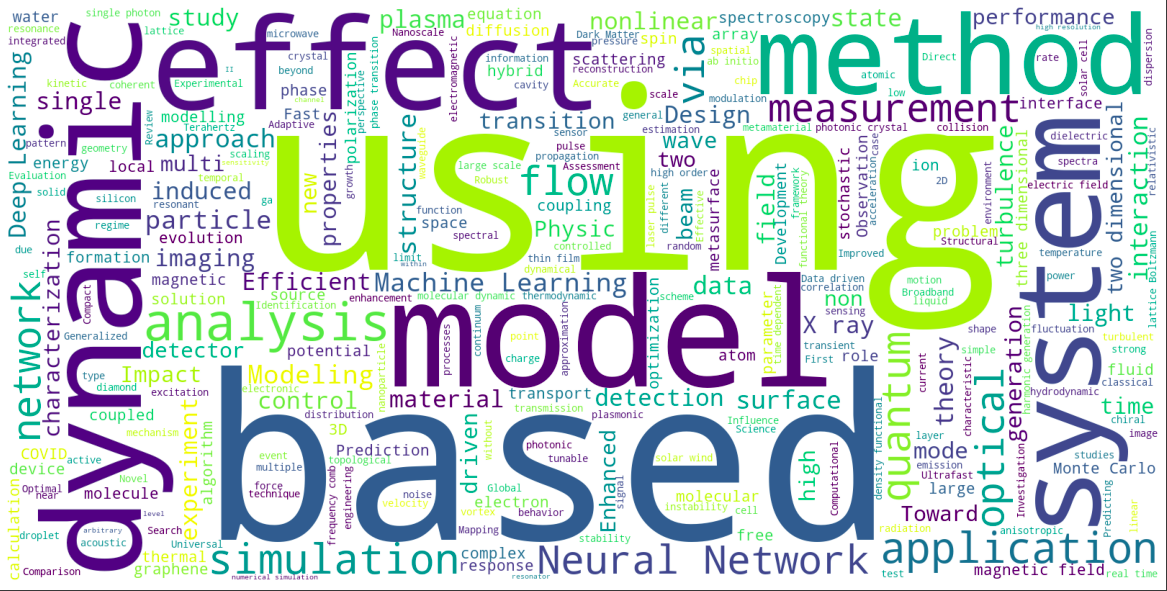
\includegraphics[scale = 0.4]{Word Cloud/physics_word_cloud.png}
    \caption{Physics Word Cloud}
    \label{fig:physics Corpus Word Cloud}
\end{figure}

\subsubsection{Inference from label based word cloud}
From cs and stat word cloud, we can see lots of similar word in both labels like model, neural network, machine learning, network, data, distribution, etc. When looking on to the abstract of these labels, just by judging through the corpus, some of them were even hard for human to classify between them. Similar was the case with astro-ph and  physics which can be clearly visualized in the word cloud.

\begin{figure}[H]
    \centering
    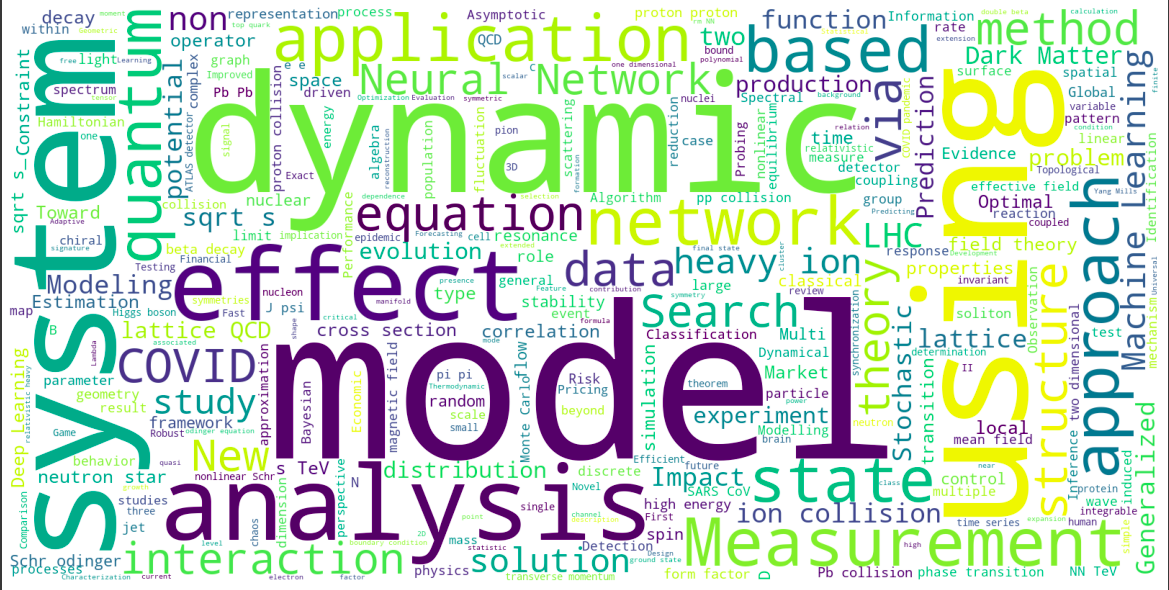
\includegraphics[scale = 0.4]{Word Cloud/minority_class_word_cloud.png}
    \caption{minority class Word Cloud}
    \label{fig:minority class Corpus Word Cloud}
\end{figure}

Minority class includes labels with number of data less than 15000 in training datasets. The classes are q-bio, hep-ex,
math-ph, nucl-th, nlin, q-fin, econ, nucl-ex, hep-lat, q-alg, funct-an,
alg-geom

\section{N-gram Exploration}
For the exploration of the most frequency unigram, stopwords were removed from the corpus created from the whole training corpus. Then, we got the count of all unique word from the corpus in a hash map. Using the hash map, we drew this bar graph by taking the top 40 most frequent words. The result is as follow : 

\begin{figure}[H]
    \centering
    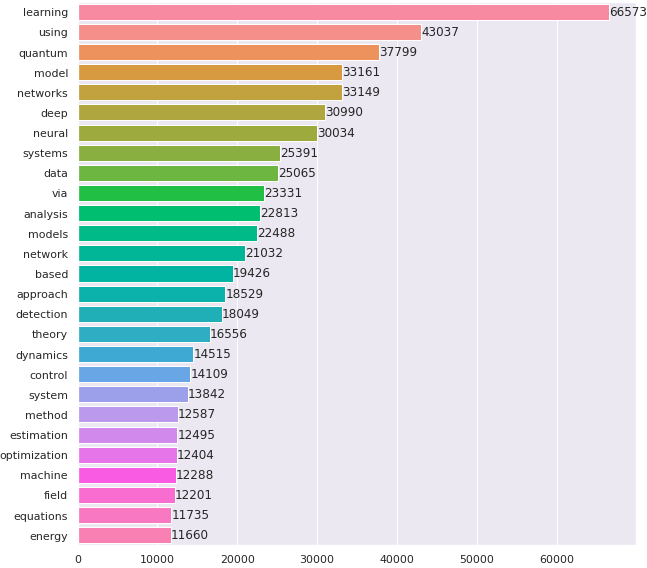
\includegraphics[scale = 0.6]{N-gram/cropped_unigram_label.png}
    \caption{Top 40 most frequent words}
    \label{fig:Top 40 most frequent words}
\end{figure}



\begin{figure}[H]
    \centering
    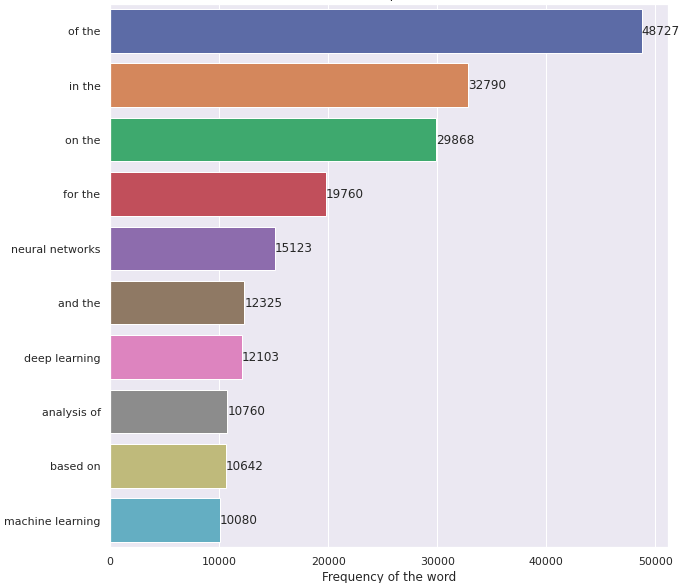
\includegraphics[scale = 0.45]{N-gram/cropped_bigram_label.png}
    \caption{Most frequent bi-grams}
    \label{fig:Most frequent bi-grams}
\end{figure}

\begin{figure}[H]
    \centering
    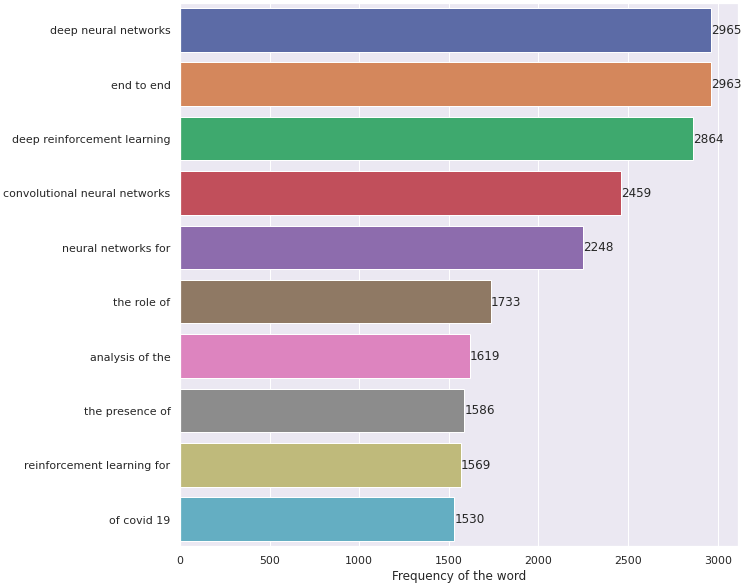
\includegraphics[scale = 0.6]{N-gram/cropped_trigram_label.png}
    \caption{Most frequent tri-grams}
    \label{fig:Most frequent tri-grams}
\end{figure}



\section{Named Entity Recognition}
\section{Part of Speech Tagging}

